\documentclass[conference]{IEEEtran}

\usepackage{graphicx}
\graphicspath{ {./images/} }

\begin{document}
	
\title{CS:GO Win/Loss prediction and feature importance for user retention}


\author{\IEEEauthorblockN{Gautam Baghel}
\IEEEauthorblockA{College of Computer and Information Science\\
Northeastern University\\
Boston, Massachusetts 02115\\}

}

\maketitle

\begin{abstract}
Computer game contributes a huge part to modern culture. Among different types of computer games, the multi-player online battle arena games generated an electronic sports community and attracted plentiful audiences.Counter Strike: GO (CS:GO), as one of the leading multi-player online battle arena games, Valve has a big responsibility on analyzing game data and improving game experiences to players.The objective is to have players stay in servers as long as possible. To achieve this we must employ a better matchmaking system which pitches the player of similar standards. In a regular server the teams are shuffled almost after every game. If the servers detect that the games are too short or the teams are unevenly matched we would need to shuffle the teams appropriately, now this is where the features will be important in deciding which players need to be employed to the other team. On completion of the maps win/loss prediction would be essential in forming the next batch of teams. This paper applies classification methods to identify the features important in winning and losing a match and also tries to predict a player's chances of winning. Through various methods of verification, the results show that features such as equipment value of both teams, rank of the victim, number of rounds and prominent maps such as \texttt{de\_dust2}, \texttt{de\_cache} and mirage are the best features in determining a player's victory.

\end{abstract}

\IEEEpeerreviewmaketitle



\section{Introduction}

In recent years, there is a rise in popularity of MOBA (Multi-Player Online Battle Arena) games. These games are usually composed of several players forming teams and competing against each other in matches. Each match can range from few minutes of play to hours of play. CS:GO alone reportedly has over 100 million monthly active users \cite{Loterina}. Professional players have made careers out of playing professional MOBA games with earnings in the range of two million dollars annually \cite{esports}. Electronic sports (eSports) are becoming an important part of our culture. In this paper, we are interested in (a) understanding what features may impact win/loss. Understanding the win/loss and matchmaking statistics has design and user experience implication, but also perhaps a learning implication. For game designers, it may be environmental elements of the game which contribute to synergy in a game. For producers, it may be involvement of more players and getting them hooked on the game. For players, it gives them an opportunity to refine their skills where it proved to be inadequate.

To achieve this goal, the paper uses a game analytics approach where data from a MOBA game is analyzed through machine learning algorithms. There has been similar work in this area. Looking at the weapon and equipments used in the games to figure out different winning strategies employed by the players. Player personalities may vary in different players altogether and the findings are preliminary. Champion type analysis only looks at the composition based on champion specific skills, player effectiveness in using the champion is not evident. Team versus star player analysis gives a better picture of cooperation versus competition in the game.  

In order to tackle this problem, we analyzed 534,398 data of team statistics from CS:GO kaggle datasets. We used analyzed all the players in terms of their contribution to winning/losing. To answer that we turned this into a classification question where we predict win/loss based on important features and slightly correlated features. This kind of analysis is the first of its kind to understand the contribution of the features inlvolved like the guns used or the damage done. The contribution is in the results that we found and it adds to previous work on team level analysis in MOBA game from a different perspective. 

This paper is divided into the following section. First, we discuss previous work in more detail outlining the open problems given the work done in MOBA games. Second, we discuss the game we used and the dataset. Third, we discuss the algorithms used and results obtained. We then discuss the results in more detail. We conclude by outlining the contribution and applications of the results.  



\section{Previous Work}
A study by Christoph Eggert and team \cite{Eggert2015} which classified players into sets of classes and segments of games with respect to their roles, effectiveness in time (early/late) and support items/ damage types. Using Logistic Regression, Random Forest and Bayesian Networks to reduce the set of player classes for better accuracy in predicting the winner. A team-based approach to MOBA is similar but on aspects divided on roles. Limitations may include predetermining roles in the game which may lead to some early misdirection in team formation.

 Personality aspects have also been taken into consideration while forming a team where the study investigated how personality trait and expertise affect virtual team interactions \cite{Balthazard2004}. Using correlation analysis, regression analysis, and a series of post hoc t-tests they were able to hypothesize the mechanisms through which personal characteristics of individuals are aggregated via group-level dynamics to produce group-level outcomes and approached the  team v/s individual performance based on personality traits. They concluded that the results were preliminary and since they were formed into interdependent teams for only the relatively brief duration of their task it cannot be used universally.

Another team analysis 'Learning Dota 2 Team Compositions' \cite{Agarwala2014}, studied teams using PCA and second order PCA with Logistic regression was done for a different MOBA game Dota 2, using hero composition. They concluded that cleaner data or better models are needed. Factors responsible may have been player skills which were not taken into consideration.

The clustering algorithm used in the paper Player Behavior and Optimal Team Composition based on champion types is done in Online Multiplayer Game study based on champion types by Hao Yi Ong and team \cite{Bainbridge2009} was effective in forming teams based on champion types. The focus in this paper is on player types like ambush-er, magic, physical, support etc. and team composition from that, whether a specific class of champions has any effect on winning. It uses clustering of players based on their behaviors, visualizing the data using PCA and predicting the winner using classification. Factors not taken into consideration was team play behaviors like assists and player skill-based classification.

Research done in similar area  Player Skill Decomposition in Multiplayer Online Battle Arenas \cite{Chen2016} looked at 14 cooperative games to find out game-play design aspects which determine the interaction between player. Their research showed that helping occurred when the game was difficult for players which may be a factor in teams which win in the league of legends. Results may be time dependent and as the game changes rapidly over the years, player strategies may have evolved differently from MOBA games. 

Making use of game log data, 'On Successful Team Formation' \cite{Pobiedina2013b} chose a statistical approach to identify factors that increase the chance of a team to win. Their hypothesis being better role distribution in a team increases the chance to win a game,     teams with more experienced players have a higher chance to win, playing with friends increases the chance to win and
the selection of a proper leader as well as a good matching of heroes inside a team positively influence the success. Using ANOVA test and Mann-Whitney-Wilcoxon-tests they were able to identify better Individual Hero Selection vs Team Hero Selection with log-linear analysis. In this approach, specific Gameplay elements not considered the part of analysis since MOBAs tend to be different from other online multiplayer games where gameplay aspects like inhibitors, dragons are quintessential to form strategies it falls short.
  
Effectiveness of Machine Learning algorithms in predicting game outcome by systematic review and compare performance of most frequently used machine learning algorithms for prediction of the match winner from the teams' drafts in DotA 2 computer game \cite{Semenov} deals with algorithms such as Naive Bayes classifier, Logistic Regression and Decision trees to validate consistency in data mining. Using the algorithms this paper comes up with standard performance metrics for players. This paper deals with different algorithms than the ones previously presented.

\section{Game and Data}
The data-set within the 1400 matches provides every successful entry of duels (or battle) that took place for a player. That is, each row documents an event when a player is hurt by another player (or World e.g fall damage). There are over 900,000 entries within more than 31500 rounds retrieved using valves API system. The game mode is called 5-vs-5 ranked matches of a solo queue which is extensively played casual or pro mode. A typical such match involves ten players who form two teams of five. The fields in the data-sets highlights include shooters and victims, event coordinates, and time stamps. The data-sets also includes static information on the match winner, player ranks before and after the match, and other miscellaneous match-level meta-data. as shown in (Fig. \ref{fig_sim}).


\begin{figure}[!t]
%\centering
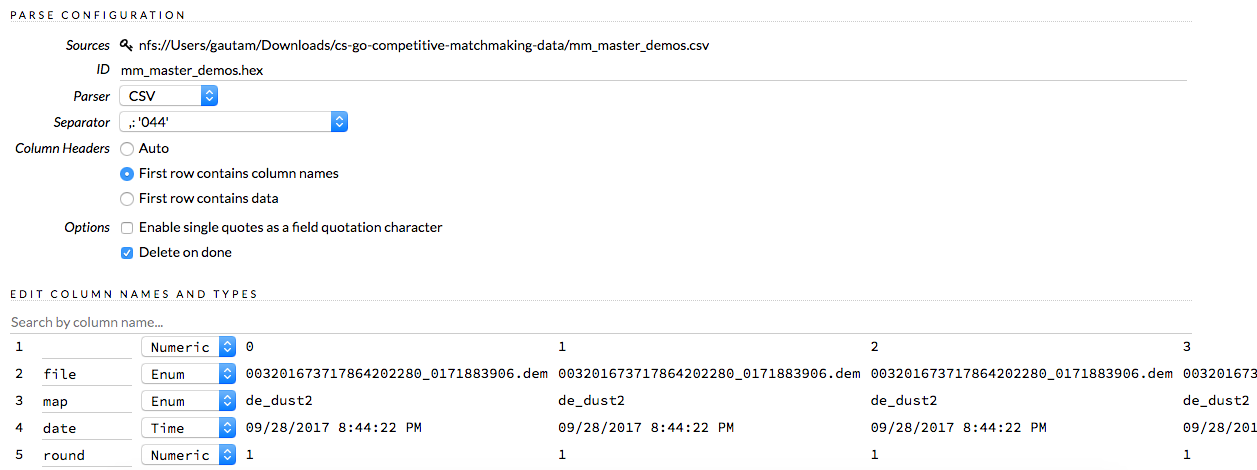
\includegraphics[width=\linewidth]{tab1.png}
% where an .eps filename suffix will be assumed under latex, 
% and a .pdf suffix will be assumed for pdflatex; or what has been declared
% via \DeclareGraphicsExtensions.
\caption{Dataset with retrieved from valve's API}
\label{fig_sim}
\end{figure}


\section{Feature Extraction}
We derived several features from the given data above: 
\begin{itemize}
  \item \textbf{Important Players}  Using backward feature selection which includes all the predictors and recursively removes the predictors which are less influential, \texttt{ct\_eq\_val} was the most important predictor with Akaike information criterion that overrules other predictors. The findings here were corroborated in the heat map of the predictors show that \texttt{ct\_eq\_val}supersedes every other predictor by considerable margins \cite{Patterson}. 
  \item \textbf{Correlation Matrix} A correlation matrix gives us a better analysis of the correlated features which need to be exempted from our analysis as it may have adverse effect on the models. The target variable winning side turned out to be highly correlated to winning team which subsided the other features.
\end{itemize}

\section{ Win/Loss and feature importance in CS:GO }


We considered and compared several methods to understand the features for predicting win/loss. 
After the separation of data set into two distinctive halves, we tried to form a learning model based on the features. The datasets comprised of categorical and quantitative data so every algorithm used had its pros and cons. When choosing reasonable methods, some dimensions are considered. For example, the number of training examples, the feature space dimensions, the relationship between features, the linearly dependent expiation between features and target variable \texttt{winner\_side}, the problem of over-fitting and the computer system’s capacity on running data analysis. Based on the dimensions we considered, these six models were chosen.

\begin{itemize}
  \item \textbf{Generalized Linear Model}
We chose this method due to we expect the CS:GO data features are roughly linear and the hypothesis problem to be linearly separable. This method is also efficient. 

In statistics, the generalized linear model (GLM) is a flexible generalization of ordinary linear regression that allows for response variables that have error distribution models other than a normal distribution. The GLM generalizes linear regression by allowing the linear model to be related to the response variable via a link function and by allowing the magnitude of the variance of each measurement to be a function of its predicted value. 

Also, since LR output can be interpreted as a probability, it proved to be good fit for the data. 

  \item \textbf{Distributed Random Forest}
Distributed Random Forest (DRF) is a powerful classification and regression tool. When given a set of data, DRF generates a forest of classification or regression trees, rather than a single classification or regression tree. Each of these trees is a weak learner built on a subset of rows and columns. More trees will reduce the variance. Both classification and regression take the average prediction over all of their trees to make a final prediction, whether predicting for a class or numeric value. (Note: For a categorical response column, DRF maps factors (e.g. ‘dog’, ‘cat’, ‘mouse) in lexicographic order to a name lookup array with integer indices (e.g. ‘cat’ - 0, ‘dog’ - 1, ‘mouse’ - 2.) 

  \item \textbf{Gradient Boosting Machine}
Gradient Boosting Machine (for Regression and Classification) is a forward learning ensemble method. The guiding heuristic is that good predictive results can be obtained through increasingly refined approximations. GBM sequentially builds regression trees on all the features of the dataset in a fully distributed way - each tree is built in parallel.

  \item \textbf{Naive Bayes}
Naïve Bayes is a classification algorithm that relies on strong assumptions of the independence of covariates in applying Bayes Theorem. The Naïve Bayes classifier assumes independence between predictor variables conditional on the response, and a Gaussian distribution of numeric predictors with mean and standard deviation computed from the training dataset.

Naïve Bayes models are commonly used as an alternative to decision trees for classification problems. When building a Naïve Bayes classifier, every row in the training dataset that contains at least one NA will be skipped completely. If the test dataset has missing values, then those predictors are omitted in the probability calculation during prediction.

  \item \textbf{Deep Learning}
  Deep Learning is based on a multi-layer feedforward artificial neural network that is trained with stochastic gradient descent using back-propagation. The network can contain a large number of hidden layers consisting of neurons with tanh, rectifier, and maxout activation functions. Advanced features such as adaptive learning rate, rate annealing, momentum training, dropout, L1 or L2 regularization, check pointing, and grid search enable high predictive accuracy. Each compute node trains a copy of the global model parameters on its local data with multi-threading (asynchronously) and contributes periodically to the global model via model averaging across the network.

  \item \textbf{Stack Ensemble}
Ensemble machine learning methods use multiple learning algorithms to obtain better predictive performance than could be obtained from any of the constituent learning algorithms. Many of the popular modern machine learning algorithms are actually ensembles. For example, Random Forest and Gradient Boosting Machine (GBM) are both ensemble learners. Both bagging (e.g. Random Forest) and boosting (e.g. GBM) are methods for ensembling that take a collection of weak learners (e.g. decision tree) and form a single, strong learner.

\begin{figure}[!t]
%\centering
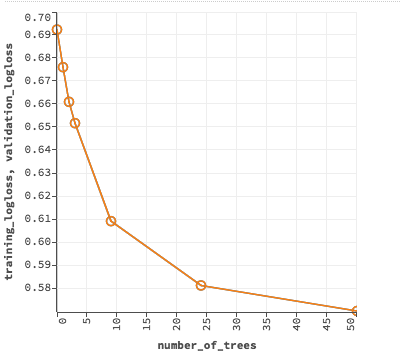
\includegraphics[width=\linewidth]{images/tab2.png}
% where an .eps filename suffix will be assumed under latex, 
% and a .pdf suffix will be assumed for pdflatex; or what has been declared
% via \DeclareGraphicsExtensions.
\caption{Tree size log loss}
%\label{fig_sim}
\end{figure}

 From the Fig. 4, 25 seems to be a good enough tree size.

\begin{figure}[!t]
%\centering
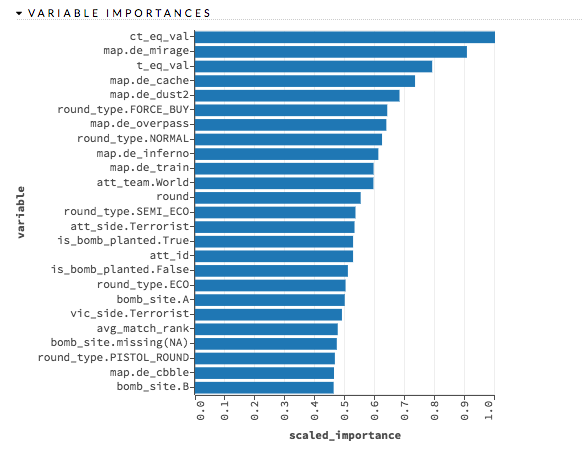
\includegraphics[width=\linewidth]{images/tab3.png}
% where an .eps filename suffix will be assumed under latex, 
% and a .pdf suffix will be assumed for pdflatex; or what has been declared
% via \DeclareGraphicsExtensions.
\caption{Feature analysis of Deep Learning}
%\label{fig_sim}
\end{figure}

\end{itemize}

\section{Results}

The validation of results is done using 10-fold cross validation method which divides the dataset into 10 subsets, and the holdout method is repeated 10 times. Each time, one of the 10 subsets is used as the test set and the other 9 subsets are put together to form a training set. Then the average error across all 10 trials is computed. The advantage of this method is that it matters less how the data gets divided. Every data point gets to be in a test set exactly once and gets to be in a training set 9 times. In every method, a confusion matrix is created 10 times for each fold. The accuracy in each of the confusion matrix is recorded and the average is considered. This method of validation is propagated across all the methods used.

Since the objective of this analysis is to  know important features and accuracy the table for the comparison of features in different algorithm is mentioned below. 
A detailed team versus star player result in is shown in table 1.

% Table generated by Excel2LaTeX from sheet 'Sheet1'
\begin{table}[htbp]
  \centering
  \caption{Comparison of all the models used}
    \begin{tabular}{|l|r|r|}
    \toprule
    Model & \multicolumn{1}{l|}{Accuracy}  \\
    \midrule
    Deep Learning   & ~0.71 \\
    \midrule
    Stack Ensemble (Boosting)   & ~0.73 \\
    \bottomrule
    \end{tabular}%
  \label{tab:addlabel}%
\end{table}%
 
The Important features

    \item \texttt{ct\_eq\_val(Numeric):} The Counter Terrorist team's total equipment value (weapon + grenades + armor + utilities) after buy time.
        Important through algorithms: Deep Learning, Gradient Boosting Machines & Naive Bayes

     \item \texttt{t\_eq\_val(Numeric):} The Terrorist team's total equipment value (weapon + grenades + armor + utilities) after buy time.
        Important through algorithms: Deep Learning, Gradient Boosting Machines & Naive Bayes

     \item \texttt{vic\_rank(Numeric):} The new rank of the victim after the match is complete. Both \texttt{att\_rank} and \texttt{vic\_rank} are constant over all damage entries for each player/match.
        Important through algorithms: Generalized Linear Model

     \item \texttt{round(Numeric):} The round that the duel took place.
        Important through algorithms: Distributed Random Forest, Generalized Linear Model

     \item \texttt{tick(Numeric):} The current tick in the demo the entry took place. A tick is represented as a state in the game, Valve's competitive matchmaking sets every match at 64 ticks which represents that there are 64 states within each second of the game.
        Important through algorithms: Distributed Random Forest

     \item \texttt{att\_rank(Numeric):} The new rank of the attacking player after the match is complete.
        Important through algorithms: Generalized Linear Model

\section{Conclusion}

The features are important because the objective is to have players stay in servers as long as possible. They're important in deciding which players need to be employed to the other team. On completion of the maps win/loss prediction would be essential in forming the next batch of teams. 

Deep Learning had the best analysis was done by the deep learning model it emphasized the particular biases in winning or losing based on maps. Mirage, \texttt{de\_cache} and \texttt{de\_dust2} were among the chief factors for people winning or loosing matches as several of the advanced player had experience playing those maps.

Another factor was 'Force Buy' in round Types, in CSGO when you lose a round you often don't have enough money to buy weapons and equipment. you will buy pistols then and go in an eco-round. a force buy is an eco-round where you have to buy because it's for example the last round in the half.

For Accuracy calculations and straight predictions of win/loss without feature importance the best algorithm would be Stack - Ensemble it has an accuracy of ~0.73. We don't wanna have a high accuracy model because if we're certain which team is going to win it's going to make the matches less interesting.

The data set also contained lots of data on map locations and bomb analysis. This paper did not delve into that consideration. Further more valve may have employed certain algorithm to perform matchmaking already which may affect this analysis.

\medskip
 
\bibliographystyle{plain}
\bibliography{mypaper_references} 

\end{document}
